
\documentclass{standalone}
\usepackage{fourier}
\usepackage{tikz}
\usetikzlibrary{shapes,shapes.misc,arrows}
\tikzset{cross/.style={cross out, draw=black, minimum size=2*(#1-\pgflinewidth), inner sep=0pt, outer sep=0pt},
%default radius will be 1pt. 
cross/.default={2pt}}
\begin{document}
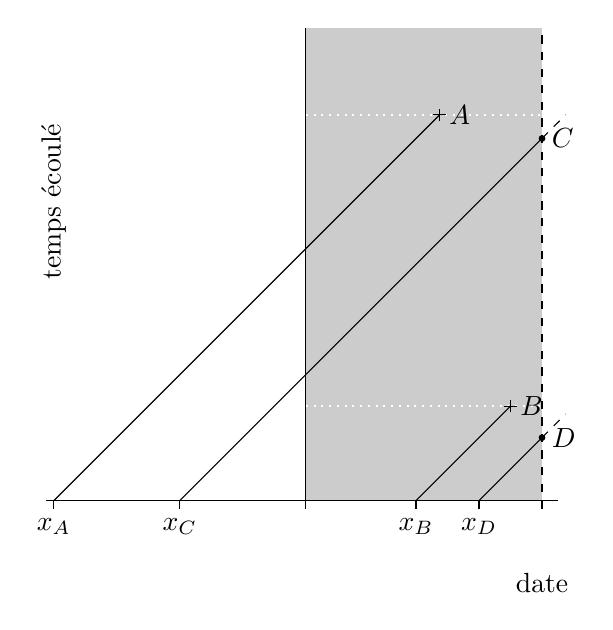
\begin{tikzpicture}

\fill [gray!40] (0,0) rectangle (3,6);
\draw[dashed](3,-0.1)--(3,6); %vertical right bar
\draw[dotted, thick, color=white](0,4.9)--(3,4.9);
\draw[dotted, thick, color=white](0,1.2)--(3,1.2);
% \draw(3.8,1.2)--(3.9,1.2) node[right] at (3.9,1.2) {$t_B$};
% \draw(3.8,0.8)--(3.9,0.8) node[right] at (3.9,0.8) {$2016-x_D$};
% \draw(3.8,1.6)--(3.9,1.6) node[right] at (3.9,1.6) {$2009-x_C$};
% \draw(3.8,3.2)--(3.9,3.2) node[right] at (3.9,3.2) {$2009-x_A$};
% \draw(3.8,4.6)--(3.9,4.6) node[right] at (3.9,4.6) {$2016-x_C$};
% \draw(3.8,4.9)--(3.9,4.9) node[right] at (3.9,4.9) {$t_A$};
% \draw (3.8,0)--(3.9,0) node[right]{$0$};

\draw (-3.3,0)--(3.2,0);
\draw (0,-0.1)--(0,6);
% \node[below] at(0,-0.1) {$2009$};
% \node[below] at(3,-0.1) {$2016$};
\draw (2.2,0)--(2.2,-0.1) node[below]at(2.2,-0.1) {$x_D$};
\draw (1.4,0)--(1.4,-0.1)  node[below] at(1.4,-0.1) {$x_B$};
\draw (-3.2,0)--(-3.2,-0.1) node[below]at(-3.2,-0.1) {$x_A$};
% Draw C
\draw (-1.6,0)--(-1.6,-0.1)  node[below]at(-1.6,-0.1) {$x_C$};
\draw (-1.6,0)-- (0,1.6);

\draw (0,1.6)-- (3,4.6);
\draw[dashed] (3,4.6) -- (3.3,4.9);
\draw[fill=black] (3,4.6) circle (1pt) ;
\node[right] at (3,4.6) {$C$};

% Draw D
\node[above left] at (-0.2,0.8) {};
\draw (2.2,0)-- (3,0.8);
\draw[fill=black] (3,0.8) circle (1pt);
\node[right] at (3,0.8) {$D$};

% Draw A
\draw[dashed] (3,0.8) -- (3.3,1.1);
\draw (-3.2,0)--(0,3.2);
\draw (0,3.2)-- (1.7,4.9);
\draw (1.7,4.9) node[cross,rotate=45] {};
\node[right] at (1.7,4.9) {$A$};
\draw (1.4,0)-- (2.6,1.2);
\draw (2.6,1.2) node[cross,rotate=45] {};
\node[right] at (2.6,1.2) {$B$};
\node [below] at (3,-0.8){date};

\node [rotate=90] at (-3.2,3.8){temps écoulé};

\end{tikzpicture}

\end{document}
